\chapter{Testing scenarios}

To test a basic scenario, two tasks have to be running at all times:
\begin{itemize}
	\item \texttt{scenario\_starter} - a process which executes scenario specific functions
	\item \texttt{UART\_test\_task} - testing (debugging) task which accepts user input as defined in Chapter \ref{ch:testing_device_fun}. It enables users to initialize scenario execution, as well as to cancel it.
\end{itemize}

Task creation is done in main function of \texttt{main.c} file. Properly setup main file to run a generic scenario is given in Figure \ref{fig:main_c}.

\begin{figure}[htb]
    \centering
	  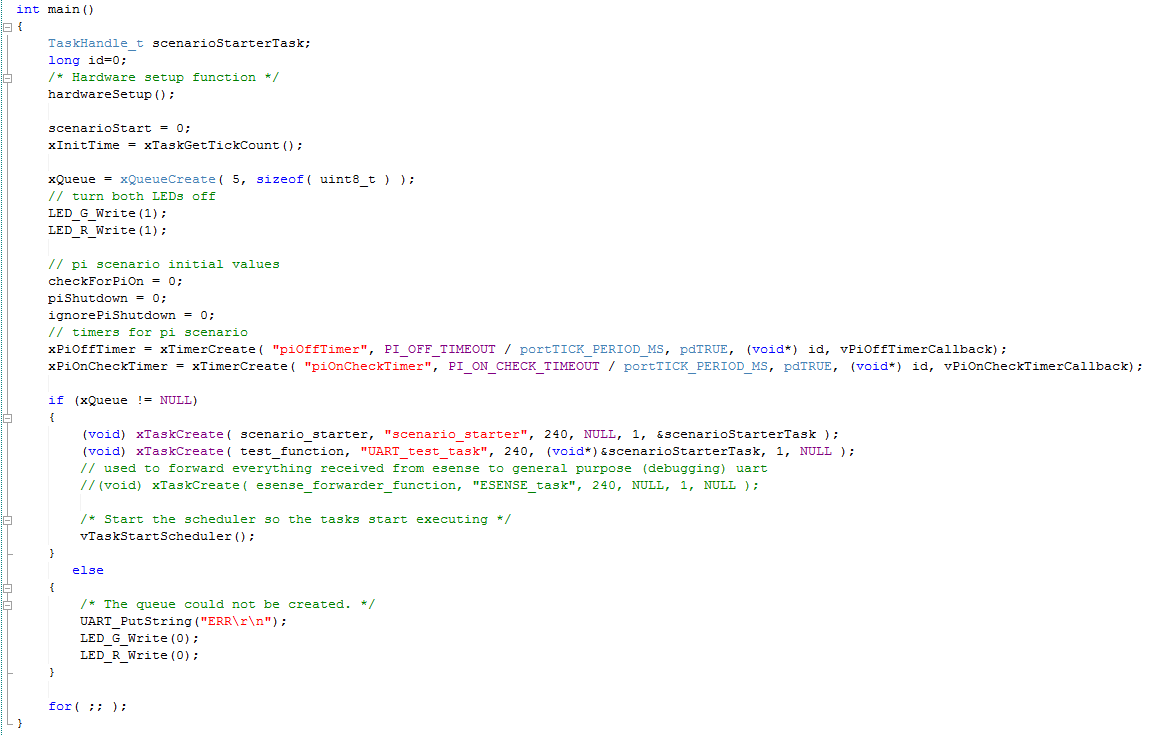
\includegraphics[width=\linewidth]{figures/Main_scenario.png}
	\caption{Main file setup to run a generic scenario}
	\label{fig:main_c}
\end{figure}

\section{Electric sense scenario}

To test electric sense, two different versions of aMussel scenario have been written -- active and passive. 

